\newpage
\section{Auswertung}
\label{sec:auswertung}
\subsection{Invertierender Linearverstärker}
    \begin{figure}[ht]
        \centering
        \includegraphics[width = 0.8\textwidth]{plots/linearVerstaerker.pdf}
        \caption{Die aus den Messwerten der Eingangs- und Ausgangsspannung berechnete Verstärkung ist in einem doppelt-logarithmischen Graphen gegen die Frequenz aufgetragen. Dabei werden nur die Messwerte im abfallenden Bereich für den Fit verwendet.}
        \label{fig:linearVerstaerker}
    \end{figure}

    Die Messwerte für \autoref{fig:linearVerstaerker} wurden aufgenommen, in dem die Frequenz verstellt wurde und am Oszilloskop alle nötigen Werte abgelesen wurden. Dabei wurde bei niedrigeren Frequenzen ein Plateaubereich in der Verstärkung sichtbar, welche anhand von \autoref{eqn:verstaerkung} berechnet wird.

    Dieser Plateaubereich wird genutzt, um die Leerlaufspannung zu bestimmen. Dies ist auf zwei Arten zu bewerkstelligen, entweder wird der Mittelwert der betroffenen Werte gebildet oder eine horizontale Ausgleichsgerade wird an die Messwerte gefittet und ihr y-Wert gibt die konstante Verstärkung an. Beide Methoden geben dabei den gleichen Wert wieder:
    \begin{equation*}
        V'_{\mathrm{const}} \approx 10,0896 \pm 0,0794
    \end{equation*}
    Mit der \autoref{eqn:reale_verstaerkung} wird dann die reale Leerlaufverstärkung
    \begin{equation*}
        V = \frac{V'_{\mathrm{const}} R_2}{R_2 - V'_{\mathrm{const}} R_1} \approx 10,0998 \pm 0,0796
    \end{equation*}
    berechnet.


    Der Fit der Exponentialfunktion
    \begin{equation*}
        V = a \cdot \nu^{b}
    \end{equation*}
    an die restlichen Messwerte im abfallenden Bereich gibt folgende Parameter wieder:
    \begin{align*}
        a &= 100,7299 \pm 5,5342 \\
        b &= -0,8364 \pm 0,0138
    \end{align*}
    Damit lässt sich die Grenzfrequenz bestimmen, die bei der Verstärkung $V' = \sqrt{2}$ definiert ist.
    \begin{equation*}
        \nu_{\mathrm{grenz}} \approx 375,0871
    \end{equation*}
    Das Bandbreitenprodukt ist somit gegeben als
    \begin{equation*}
        \nu_{\mathrm{grenz}} \cdot V'_{\mathrm{const}} \approx 3784,4932 \;.
    \end{equation*}   

    \begin{figure}[ht]
        \centering
        \includegraphics[width = 0.75\textwidth]{plots/linearVerstaerkerPhase.pdf}
        \caption{Die Phase zwischen ein- und ausgehender Spannung ist gegen die Frequenz aufgetragen. Hierzu wurden zwei Messreihen durchgeführt.}
        \label{fig:linearVerstaerkerPhase}
    \end{figure}

    Zur Betrachtung der Phase zwischen ein- und ausgehender Spannung wurden zwei Messreihen aufgenommen.

\newpage
\subsection{Umkehr-Integrator und Invertierender Differenzierer}

    Hierbei wurde beim fitten der Messwerte genauso verfahren wie bei dem Graphen zum Linearverstärker.
    Die Exponentialfunktion
    \begin{equation*}
        U_A = a \cdot \nu^{b}
    \end{equation*}
    wurde in beiden Fällen, beim Integrator, als auch beim Differenzierer, an die Messwerte gefittet.
    Dabei ergaben sich die Parameter
    \begin{align*}
        a &= 1,6545 \pm 0,2087 \\
        b &= -0,8692 \pm 0,0465
    \end{align*}
    für den Umkehr-Integrator und die Parameter
    \begin{align*}
        a &= 46,8963 \pm 11,6845 \\
        b &= 1,3808 \pm 0.2002
    \end{align*}
    für den invertierenden Differenzierer.

    \par
    Danach wurden anhand von Bildern des Bildschirms eines Oszilloskops verdeutlicht wie die beiden Schaltungen funktionieren.
    Beim Integrator sollte sich die Dreiecksspannung abrunden, die Rechteckspannung zur Dreiecksspannung werden und das sinusförmige Signal seine Form beibehalten und nur seine Phase verändern.

    Beim Differenzierer sollte die Dreiecksspannung zur Rechteckspannung werden, aus der Rechteckspannung sollte ein Signal entstehen, dass Peaks dort hat, wo das Rechteckspannungssignal Flanken und die Sinusspannung sollte zur Dreiecksspannung werden.

    Die Bilder mit der Dreiecks- und Rechteckspannung decken sich einwandfrei mit der Theorie.
    Bei dem sinusförmigen Signal können auch Veränderungen festgestellt werden, nur sind diese dort nicht so markant.

    \begin{figure}
        \centering
        \begin{subfigure}[b]{0.5\textwidth}
            \centering
            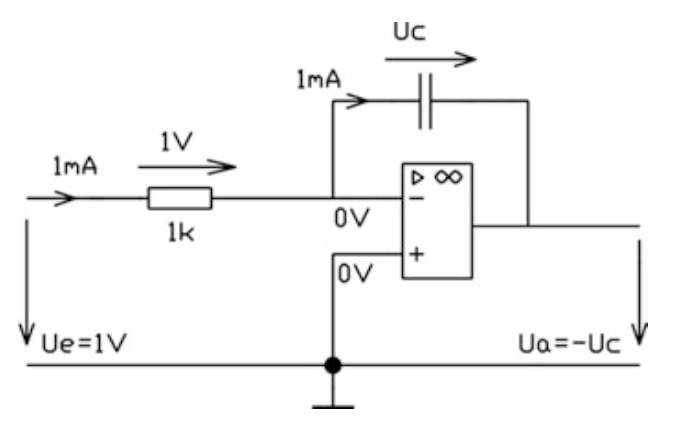
\includegraphics[width =\textwidth]{plots/integrator.pdf}
            \caption{Die Ausgangsspannung des Integrators ist gegen die Frequenz der Eingangsspannung aufgetragen und im niedrigen Frequenzbereich wurde ein Fit durchgeführt.}
            \vspace*{2cm}
            \label{fig:integrator1}
        \end{subfigure}

        \begin{subfigure}[b]{0.5\textwidth}
            \centering
            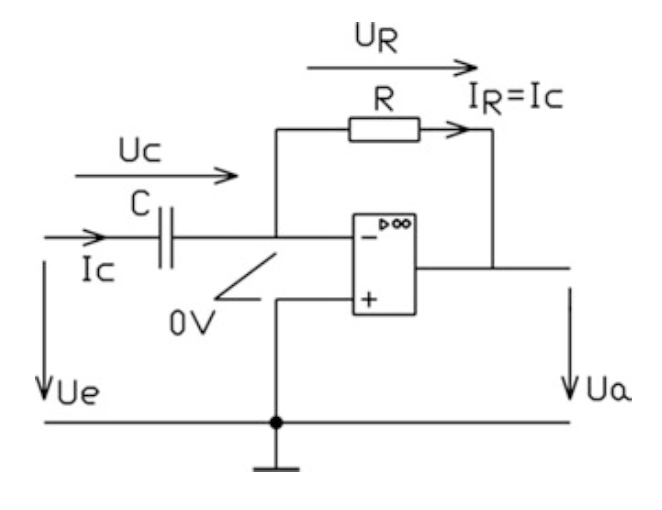
\includegraphics[width =\textwidth]{plots/differenzierer.pdf}
            \caption{Die Ausgangsspannung des Differenzierers ist gegen die Frequenz der Eingangsspannung aufgetragen und im niedrigen Frequenzbereich wurde ein Fit durchgeführt.}
            \label{fig:differenzierer1}
        \end{subfigure}
    \end{figure}
    \FloatBarrier

    \begin{figure}
        \centering
        \begin{subfigure}[b]{0.48\textwidth}
            \centering
            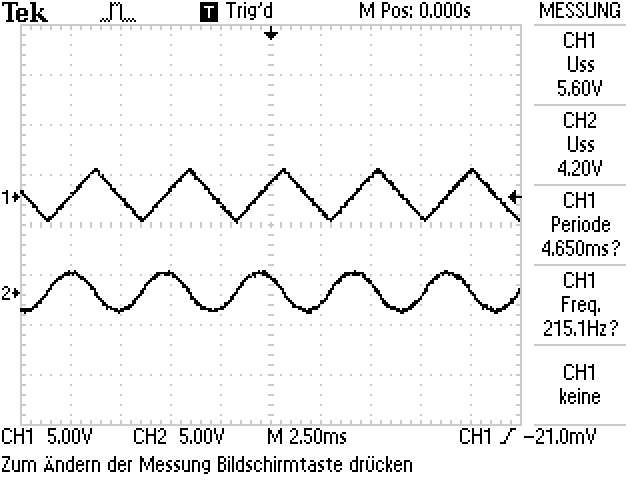
\includegraphics[width=\textwidth]{bilder/integrator_dreieck.JPG}
            \caption{Signal des Integrators bei dreieckförmiger Eingangsspannung.}
            \vspace*{1cm}
            \label{fig:integrator_dreieck}
        \end{subfigure}
    
        \begin{subfigure}[b]{0.48\textwidth}
            \centering
            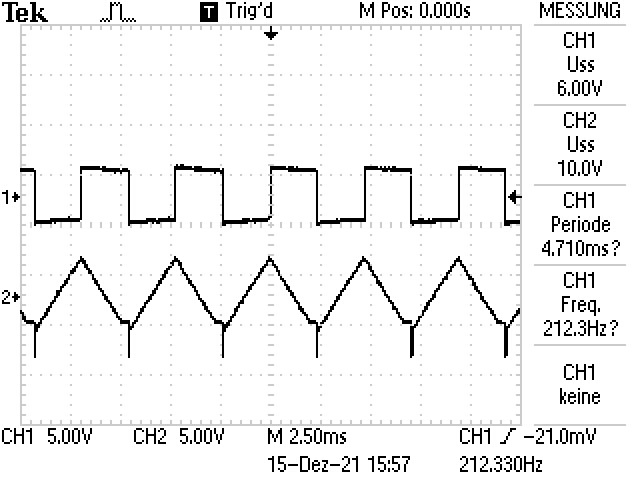
\includegraphics[width=\textwidth]{bilder/integrator_rechteck.JPG}
            \caption{Signal des Integrators bei rechteckförmiger Eingangsspannung.}
            \vspace*{1cm}
            \label{fig:integrator_rechteck}
        \end{subfigure}

        \begin{subfigure}[b]{0.48\textwidth}
            \centering
            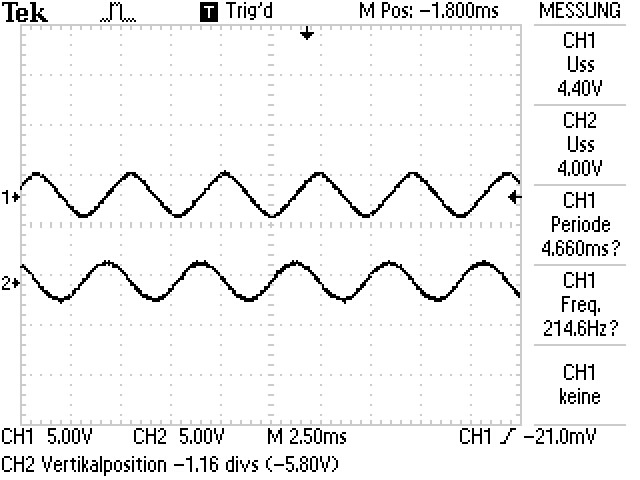
\includegraphics[width=\textwidth]{bilder/integrator_sinus.JPG}
            \caption{Signal des Integrators bei sinusförmiger Eingangsspannung.}
            \label{fig:integrator_sinus}
        \end{subfigure}
        \caption{Das ausgegebene Signal des Integrators, wenn die oben angegebenen Signale eingespeist werden.}
        \label{fig:integrator_signale}
    \end{figure}
    \FloatBarrier

    \begin{figure}
        \centering
        \begin{subfigure}[b]{0.48\textwidth}
            \centering
            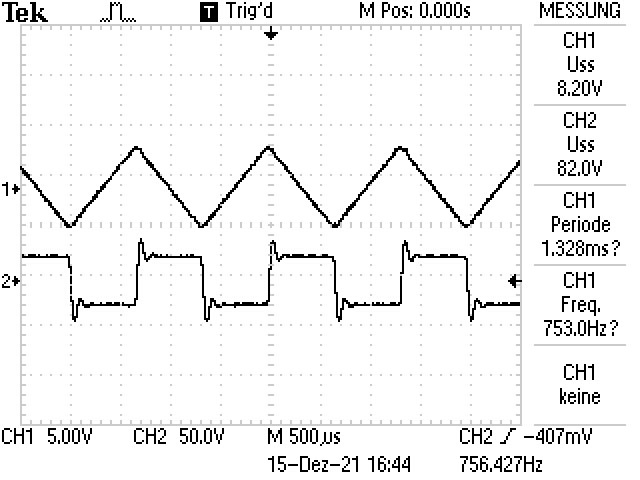
\includegraphics[width=\textwidth]{bilder/differenzierer_dreieck.JPG}
            \caption{Signal des Differenzierers bei dreieckförmiger Eingangsspannung.}
            \vspace*{1cm}
            \label{fig:differenzierer_dreieck}
        \end{subfigure}
    
        \begin{subfigure}[b]{0.48\textwidth}
            \centering
            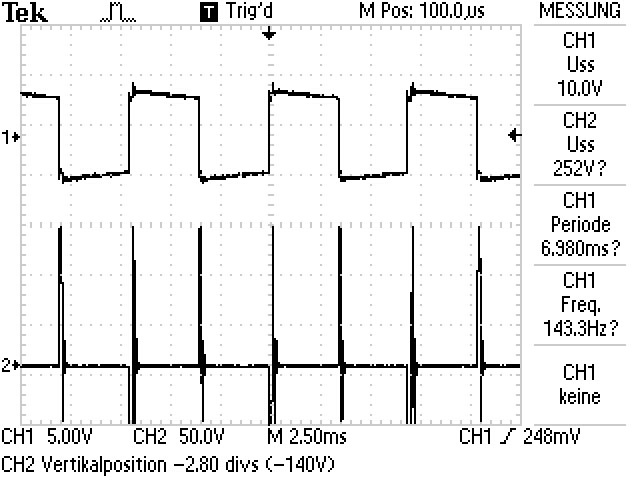
\includegraphics[width=\textwidth]{bilder/differenzierer_rechteck.JPG}
            \caption{Signal des Differenzierers bei rechteckförmiger Eingangsspannung.}
            \vspace*{1cm}
            \label{fig:differenzierer_rechteck}
        \end{subfigure}

        \begin{subfigure}[b]{0.48\textwidth}
            \centering
            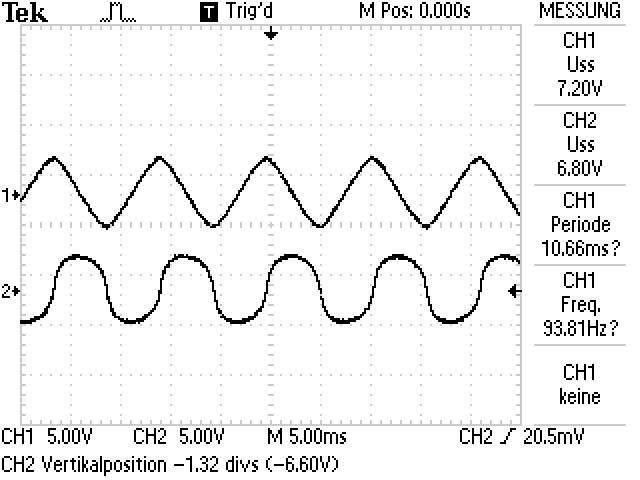
\includegraphics[width=\textwidth]{bilder/differenzierer_sinus.JPG}
            \caption{Signal des Differenzierers bei sinusförmiger Eingangsspannung.}
            \label{fig:differenzierer_sinus}
        \end{subfigure}
        \caption{Das ausgegebene Signal des Differenzierers, wenn die oben angegebenen Signale eingespeist werden.}
        \label{fig:differenzierer_signale}
    \end{figure}
    \FloatBarrier

